\documentclass{sigchi}

% Use this command to override the default ACM copyright statement
% (e.g. for preprints).  Consult the conference website for the
% camera-ready copyright statement.


%% EXAMPLE BEGIN -- HOW TO OVERRIDE THE DEFAULT COPYRIGHT STRIP -- (July 22, 2013 - Paul Baumann)
% \toappear{Permission to make digital or hard copies of all or part of this work for personal or classroom use is      granted without fee provided that copies are not made or distributed for profit or commercial advantage and that copies bear this notice and the full citation on the first page. Copyrights for components of this work owned by others than ACM must be honored. Abstracting with credit is permitted. To copy otherwise, or republish, to post on servers or to redistribute to lists, requires prior specific permission and/or a fee. Request permissions from permissions@acm.org. \\
% {\emph{CHI'14}}, April 26--May 1, 2014, Toronto, Canada. \\
% Copyright \copyright~2014 ACM ISBN/14/04...\$15.00. \\
% DOI string from ACM form confirmation}
%% EXAMPLE END -- HOW TO OVERRIDE THE DEFAULT COPYRIGHT STRIP -- (July 22, 2013 - Paul Baumann)


% Arabic page numbers for submission.  Remove this line to eliminate
% page numbers for the camera ready copy 

%\pagenumbering{arabic}

% Load basic packages
\usepackage{balance}  % to better equalize the last page
\usepackage{graphics} % for EPS, load graphicx instead 
%\usepackage[T1]{fontenc}
\usepackage{txfonts}
\usepackage{times}    % comment if you want LaTeX's default font
\usepackage[pdftex]{hyperref}
% \usepackage{url}      % llt: nicely formatted URLs
\usepackage{color}
\usepackage{textcomp}
\usepackage{booktabs}
\usepackage{ccicons}
\usepackage{todonotes}
\usepackage{soul}
\usepackage{paralist}

\usepackage{caption}
\usepackage{subcaption}
\usepackage[super]{nth}
\usepackage{amsmath}

% llt: Define a global style for URLs, rather that the default one
\makeatletter
\def\url@leostyle{%
  \@ifundefined{selectfont}{\def\UrlFont{\sf}}{\def\UrlFont{\small\bf\ttfamily}}}
\makeatother
\urlstyle{leo}

% To make various LaTeX processors do the right thing with page size.
\def\pprw{8.5in}
\def\pprh{11in}
\special{papersize=\pprw,\pprh}
\setlength{\paperwidth}{\pprw}
\setlength{\paperheight}{\pprh}
\setlength{\pdfpagewidth}{\pprw}
\setlength{\pdfpageheight}{\pprh}

% Make sure hyperref comes last of your loaded packages, to give it a
% fighting chance of not being over-written, since its job is to
% redefine many LaTeX commands.
\definecolor{linkColor}{RGB}{6,125,233}
\hypersetup{%
  pdftitle={SIGCHI Conference Proceedings Format},
  pdfauthor={LaTeX},
  pdfkeywords={SIGCHI, proceedings, archival format},
  bookmarksnumbered,
  pdfstartview={FitH},
  colorlinks,
  citecolor=black,
  filecolor=black,
  linkcolor=black,
  urlcolor=linkColor,
  breaklinks=true,
}

% create a shortcut to typeset table headings
% \newcommand\tabhead[1]{\small\textbf{#1}}

% End of preamble. Here it comes the document.
\begin{document}

\title{Measuring Interaction Design\\
Measuring Interaction before developing prototypes\\
Measuring Interaction Graphs}

\numberofauthors{2}
\author{%
  \alignauthor{1st Author Name\\
    \affaddr{Affiliation}\\
    \affaddr{City, Country}\\
    \email{e-mail address}}\\
  \alignauthor{2nd Author Name\\
    \affaddr{Affiliation}\\
    \affaddr{City, Country}\\
    \email{e-mail address}}\\
}

\maketitle

\begin{abstract}
  Early development of prototypes is good practice for user interface
  development. However, they have to cover specific usage scenarios,
  and because they are limited in focus, the whole picture of the user
  interface is easily lost. Even simple questions dealing with
  numerosity and length of execution paths or impact of possible user
  errors can be answered only for the specific scenarios being
  analysed.

  We discuss a tool that transforms models of a user interface into a
  graph. This is then used to specify usage scenarios, and to generate
  possible execution traces. Metrics based on different possible
  execution paths, with or without possible mistakes, can be easily
  computed. When applying these metrics to Gmail and Roundcube in a
  typical scenario, we learn for example that Gmail has 7 times more
  optimal paths, it has 4x more paths include at most one possible
  user error, that it has 20\% fewer steps.
  
\end{abstract}

\keywords{Experimental; Evaluation; Statecharts: UML; UML-IDEA; Testing.}

\category{H.5.1}{Information interfaces and presentation (e.g., HCI)}{Multimedia Information Systems}. 
\category{H.5.2}{Information interfaces and presentation (e.g.,
  HCI)}{User Interfaces}. 

\section{Introduction}

\begin{quote}
  Subcommittee: Technology, Systems, and Engineering

People we should pay particular attention to:
Caroline Appert
Conversy, St�phane
Nebeling, Michael

Keyword we need to pay attention to:
This subcommittee will focus on technology, systems and engineering
contributions that enable, improve, or advance interaction. This will
include software and hardware technologies and systems that enable and
demonstrate novel interactive capabilities, as well as languages,
methods and tools for construction and engineering of interactive
systems. Engineering contributions should clearly demonstrate how they
address interactive systems concerns such as, for example,
scalability, reliability, interoperability, testing, and
performance. Systems and technology contributions will be judged by
their technical innovation and/or ability to connect, simplify or
enrich interactions, for example in intelligent interfaces and
mobile/ubiquitous computing.

\end{quote}


We present an approach that allows a designer to quickly 
\begin{inparaenum}[(a)]
\item understand how supportive an application is with respect to  user efficiency;
\item understand how prone the application is to user navigation
  errors;
\item understand how recoverable the application is from those errors;
\item support task analysis and task / scenario design.
%\item support interaction design (IxD) in terms of consistency, error-proneness, and recovery premature commitment;
\end{inparaenum}
%
Our approach further allows different designs to be objectively
compared to support designers in evaluating interaction sequences. To
explain our work we present (\S~\nameref{sec:casestudy}) a case study
comparing four different web mail front ends. We have chosen this
domain because it is very well understood by readers and yet those
trivial questions lead to non trivial results.

The approach is based on UML state-chart models of the user interfaces
which are automatically processed to produce \emph{interaction
  graphs}. These are then used to unfold \emph{execution traces} that
are dependent on the specific usage scenarios being considered in the
analysis (\S~\nameref{sec:traces}). On traces several graph-theoretic
computations can be performed to produce a dashboard of different
results that provide the answers. Except for development of models and
specification of the desired scenarios, the other steps are totally
automatic; models of a design could be developed in a matter of a
couple of hours.

Developing good user interfaces for web or mobile applications is a
complex and expensive endeavour. One reason is the combination of
devices, interaction modalities and workflows that need to be
supported.

Adopting Usage Centred Development practices is effective, as is
following established design principles~\cite{constantine99}. Early
prototyping~\cite{buxton07} to explore part of the five-dimensional
prototyping space~\cite{mccurdy06} is one of the most effective
techniques, especially when paired with usability investigations based
on user testing or heuristic evaluations.

However, it still requires development of prototypes that are usually
developed with certain tasks in mind, and therefore are quite
restricted in terms of depth and breadth of supported use
cases. Furthermore, usability results are always surrounded by a cloud
of uncertainty, due to subjectivity introduced by participants and
facilitators or by other contingency factors involved in the
analysis. Thus, although an effort needs to be expended to develop and
use prototypes, less than optimal results are obtained.

A designer, while conceiving and developing a solution, might benefit
from answers to seemingly simple questions that should not require a
significant investment of time and effort. For example, given one or more potential
solutions and some usage scenarios, interesting questions could
include: ``How many different ways can be followed to carry out the
scenario?'', ``Which are the shortest ones?'', ``If a user makes a
mistake, would he or she be able to recover?'', ``How many steps
would the recovery require?''. For example, when designing and
evaluating embedded user interfaces (such as when dealing with plane's
cockpits~\cite{conversy07}), other relevant questions might include
``How would the above properties change if we add a certain a
widget?'', or ``... if we replace a widget with another?''.  At the
moment, even these straightforward questions are quite complex to
answer. In fact, they require inspection of prototypes, manual
tracking of which screens and widgets are used at which stage, and
exhaustive searches.

This should not be the case, however. These answers provide important
insights to a designer, and support decisions related to benchmarking
different solutions, to identification of optimal or mistaken paths,
to assessment of suitability of a design with respect to scenarios.

Our contribution consists of the development of a tool that transforms
models and scenario specifications into execution traces, and the
definition of metrics that provide concise, precise and objective
measures of a design. The case study we illustrate shows that among
four web mail applications, and with respect to a  typical usage
scenario, Gmail has the largest number of shortest sequences of steps
(even when users are supposed to make 1 or 2 mistakes), but when users
make more than 2 mistakes the number drops significantly; on average,
best and worst cases, Gmail features also shorter paths, requiring 20\%
fewer steps; however, the probability that a user hits an optimal path
with Gmail is almost half of that of another application. All these
values suggest that Gmail offers more  efficient options to
accomplish tasks included in the scenario, but that it might be more
difficult for novice users to exploit the most efficient
methods. Further inspections show that some differences are due to the
slightly different interaction structures adopted for uploading messages.

\section{Background}
\label{sec:background}

(right now these are random notes)

SwingState: work done by 
Caroline Appert\cite{appert2008swingstates}

in java, FSA used as a conceptual framework to write the code of
widgets so that events and event handlers in the ui can more easily be
conceived, developed and verified.

They say: StateCharts were used in the StateMaster User Interface
Management System [40], and a variant of them specifically tailored to
designing user interfaces was used in the more recent HsmTk toolkit
[18]. StateCharts however are significantly more complicated and hard
to learn than plain state machines, and our experience is that user
interface designers and developers have difficulties exploiting their
power. Other approaches include Petri Nets [41], which have also been
used to specify user interfaces, for example in the PetShop system
[42]. Here too, the learning curve is steep, making the adoption of
such a model by developers difficult.

With SwingStates, any number of state machines can run simulateneously. A state machine
can be active, i.e., handling the events it receives, or inactive,
i.e., ignoring events

We adopt a similar apporach, but using UML state machine (which are
more powerful than FSA) for conceiving, guiding development, analysis
and verification of the behavior of the entire app.

Nebeling says:\cite{nebeling2011metrics}

Despite the fact that screen sizes and average screen resolutions have
dramatically increased over the past few years, little attention has
been paid to the design of web sites for large, high-resolution
displays that are now becoming increasingly used both in enterprise
and consumer spaces. We present a study of how the visual area of the
browser window is currently utilised by news web sites at different
widescreen resolutions. The analysis includes measurements of space
taken up by the article content, embedded ads and the remaining
components as they appear in the viewport of the web browser. The
results show that the spatial distribution of page elements does not
scale well with larger viewing sizes, which leads to an increasing
amount of unused screen real estate and unnecessary scrolling. We
derive a number of device-sensitive metrics to measure the quality of
web page layout in different viewing contexts, which can guide the
design of flexible layout templates that scale effectively on large
screens.

Stephane Conversy\cite{conversy07} says: (friend of nicolas roussel in
the committee)

ARINC 661 provides precise information for communication protocol
between application (called User Applications) and user interface
components (called widgets) as well as precise information about the
widgets themselves. However, in ARINC 661, no information is given
about the behaviour of these widgets and about the behaviour of an
application made up of a set of such widgets.

The purpose of ARINC 661 specification (ARINC 661, 2002) is to define
interfaces to a Cockpit Display System (CDS) used in interactive
cockpits that are now under

application of a formal description technique to the various elements
of ARINC 661 specification within an industrial project. This formal
description technique called Interactive Cooperative Objects defines
in a precise and non-ambiguous way all the elements of ARINC 661
specification. The application of the formal description techniques is
shown on an interactive application called MPIA (Multi Purpose
Interactive Application). Within this application, we present how ICO
are used for describing interactive widgets, User Applications and
User Interface servers (in charge of interaction techniques). The
emphasis is put on the model-based management of the feel of the
applications allowing rapid prototyping of the external presentation
and the interaction techniques.

The Interactive Cooperative Objects (ICOs) formalism is a formal
description technique dedicated to the specification of interactive
systems [4, 11]. It uses concepts borrowed from the object-oriented
approach to describe the structural or static aspects of systems, and
uses high-level Petri nets [8] to describe their dynamic or
behavioural aspects.

The Interactive Cooperative Objects (ICOs) formalism is a formal
description technique dedicated to the specification of interactive
systems [4, 11]. It uses concepts borrowed from the object-oriented
approach to describe the structural or static aspects of systems, and
uses high-level Petri nets [8] to describe their dynamic or
behavioural aspects.

Voida\cite{voida} says:
We describe an alternative model for organizing the
desktop interface-activity-based computing-and
identify a series of high-level system requirements for
interfaces that use activity as their primary organizing
principle.

We could mention this work when we introduce scenarios, and say that
people inventing these new metaphors could take advantage of our
metrics if they model 2+ apps. 

Eg. they say: Requirement 2. Activity-based systems should provide
lightweight mechanisms to create, change, and alter
activities, since heavyweight interaction techniques are
likely to deter adoption and use.

eg Requirement 7. Because information sharing is a
�common case� in knowledge work, lightweight sharing
capabilities should be integrated directly as a first-class
interaction technique. 

\section{Generation of execution traces}
\label{sec:traces}

\begin{quote}
  here we describe how we transform state machines into graphs, how we
  specify scenarios, how the system computes traces, how metrics are
  computed. 
\end{quote}


\section{A case study}
\label{sec:casestudy}

\subsection{Models and scenarios}
\label{sec:models-scenarios}



\subsection{Results}
\label{sec:results}


\clearpage

\begin{figure}
  \centering
  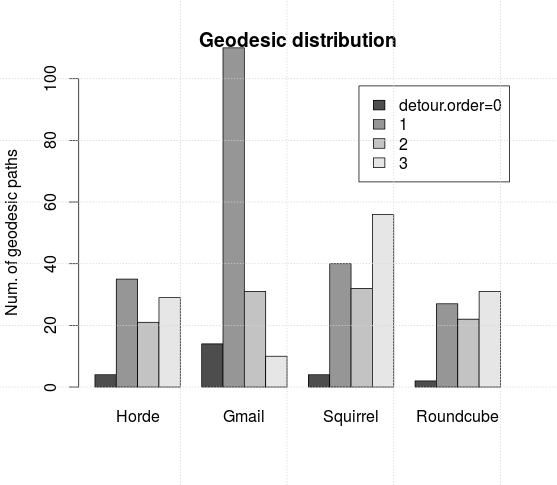
\includegraphics[width=\linewidth]{figures/num-paths.png}
  \caption{Number of geodesic paths split by detour order.}
\end{figure}


\begin{figure}
  \centering
  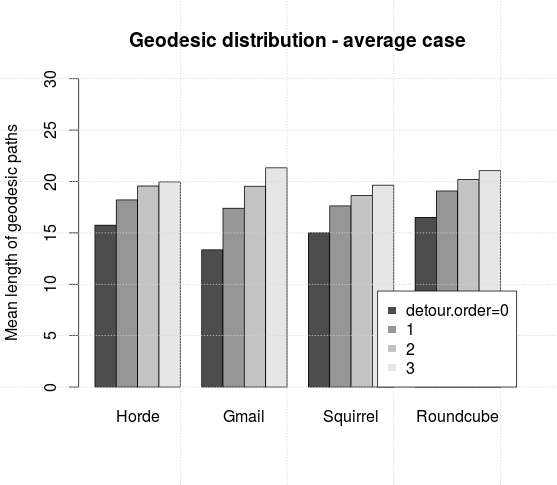
\includegraphics[width=\linewidth]{figures/averagecase.png}
  \caption{Average length of  geodesic paths split by detour order.}
\end{figure}

\begin{figure}
  \centering
  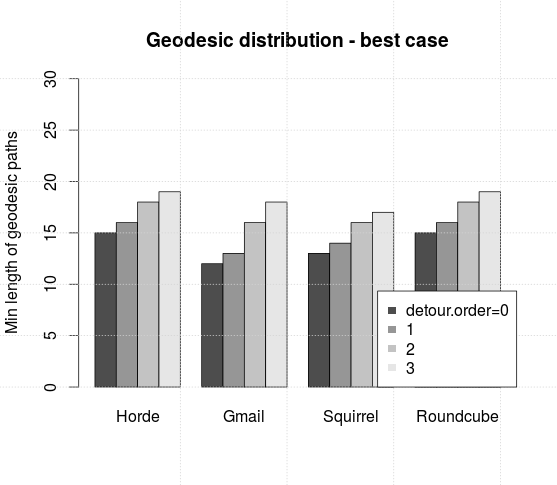
\includegraphics[width=\linewidth]{figures/bestcase.png}
  \caption{Minimum length of geodesic paths split by detour order.}
\end{figure}


\begin{figure}
  \centering
  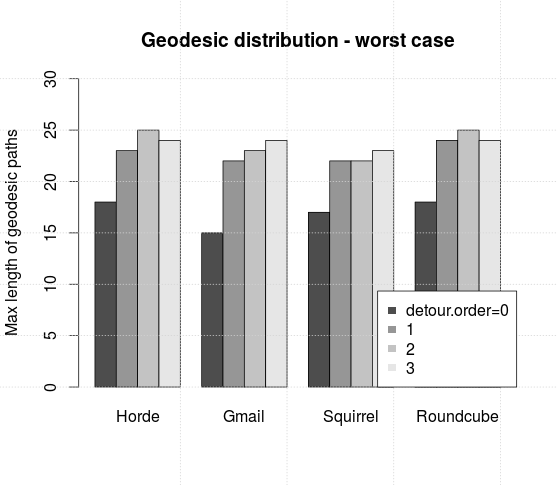
\includegraphics[width=\linewidth]{figures/worstcase.png}
  \caption{Maximum length of geodesic paths split by detour order.}
\end{figure}


\begin{figure}
  \centering
  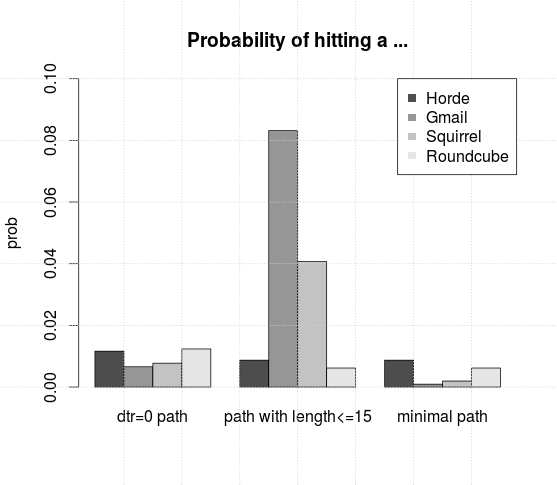
\includegraphics[width=\linewidth]{figures/prob-opt-path.png}
  \caption{Frequency of an optimal path.}
\end{figure}

\begin{figure}
  \centering
  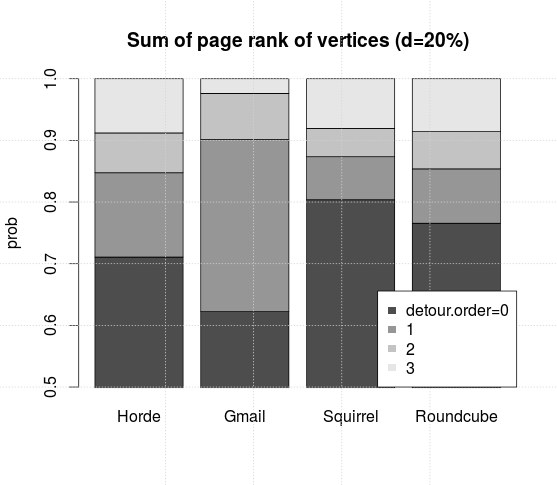
\includegraphics[width=\linewidth]{figures/pr.png}
  \caption{Probability that a random walk visit detour 0, 1, 2 or 3 states.}
\end{figure}

\section{Discussion}
\label{sec:discussion}

\section{Conclusion}
\label{sec:conclusion}





% REFERENCES FORMAT
% References must be the same font size as other body text.
\bibliographystyle{SIGCHI-Reference-Format}
\bibliography{gb,database}

\end{document}

%%% Local Variables:
%%% mode: latex
%%% TeX-master: t
%%% End:
